\documentclass[leqno]{article}
\usepackage[utf8]{inputenc}
\usepackage{enumitem}
\usepackage{tikz}
\usepackage[parfill]{parskip} % Don't start new paragraph with tab.
\usepackage{amsmath} % For \tag and \eqref

\title{Computationele logica}
\author{
    \small Kamans, Jim\\
    \texttt{10302905}
    \and
    \small Hendrikse, Mila\\
    \texttt{00000000}
    \and
    \small Roosingh, Sander\\
    \texttt{11983957}
    \and
    \small Schenk, Stefan\\
    \texttt{11881798}
}
\date{November 2017}

\begin{document}

\maketitle


%%%%%%%%%%%%%%%%
%% Exercise 1 %%
%%%%%%%%%%%%%%%%
\section{Exercise 1}

\begin{enumerate}

    \item The sentence $\theta$ encoding all information: \\

    The Queen knows the following: \\
    Alice knows Bob has a red hat. Alice knows Bob doesn't know it, and she knows the Queen knows this. Alice doesn't know her own hat. \\
    Bob knows Alice has a red hat. Bob knows Alice doesn't know it, and he knows the Queen knows this. Bob doesn't know his own hat. \\

    $\theta$ =
        $K_q (
        K_a (
            r_b \wedge
            \neg K_b (r_b \vee w_b) \wedge
            K_q ((r_a \vee r_w) \wedge (r_b \vee r_w))
        )
        \wedge \neg K_a (r_a \vee w_a)
        \wedge
        K_b (
            r_a \wedge
            \neg K_a (r_a \vee w_a) \wedge
            K_q ((r_a \vee r_w) \wedge (r_b \vee r_w))
        )
        \wedge \neg K_b (r_b \vee w_b)
        )$

    \item A representation of the situation model \textbf{M}: \\

    $\mathcal{A}$ = \{a, b, q\} the agents Alice, Bob, and the Queen \\
    $\Phi$ = $\{r_a, w_a, r_b, w_b\}$ written as WR for: a is white and b is red \\

    \begin{center}
    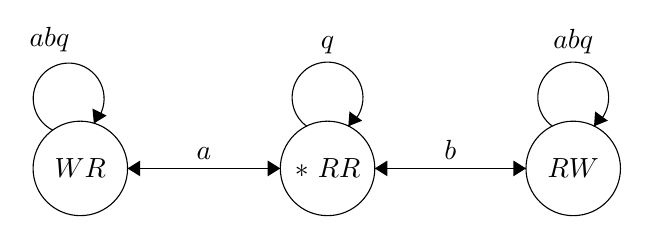
\begin{tikzpicture}[scale=0.2]
    \tikzstyle{every node}+=[inner sep=0pt]
    \draw [black] (38.4,-13.7) circle (3);
    \draw (38.4,-13.7) node {$*\mbox{ }RR$};
    \draw [black] (54,-13.7) circle (3);
    \draw (54,-13.7) node {$RW$};
    \draw [black] (22.7,-13.7) circle (3);
    \draw (22.7,-13.7) node {$WR$};
    \draw [black] (41.4,-13.7) -- (51,-13.7);
    \fill [black] (51,-13.7) -- (50.2,-13.2) -- (50.2,-14.2);
    \draw (46.2,-13.2) node [above] {$b$};
    \draw [black] (51,-13.7) -- (41.4,-13.7);
    \fill [black] (41.4,-13.7) -- (42.2,-14.2) -- (42.2,-13.2);
    \draw [black] (35.4,-13.7) -- (25.7,-13.7);
    \fill [black] (25.7,-13.7) -- (26.5,-14.2) -- (26.5,-13.2);
    \draw (30.55,-13.2) node [above] {$a$};
    \draw [black] (25.7,-13.7) -- (35.4,-13.7);
    \fill [black] (35.4,-13.7) -- (34.6,-13.2) -- (34.6,-14.2);
    \draw [black] (37.077,-11.02) arc (234:-54:2.25);
    \draw (38.4,-6.45) node [above] {$q$};
    \fill [black] (39.72,-11.02) -- (40.6,-10.67) -- (39.79,-10.08);
    \draw [black] (52.677,-11.02) arc (234:-54:2.25);
    \draw (54,-6.45) node [above] {$abq$};
    \fill [black] (55.32,-11.02) -- (56.2,-10.67) -- (55.39,-10.08);
    \draw [black] (20.955,-11.274) arc (243.46232:-44.53768:2.25);
    \draw (20.74,-6.36) node [above] {$abq$};
    \fill [black] (23.56,-10.84) -- (24.37,-10.35) -- (23.47,-9.9);
    \end{tikzpicture}
    \end{center}

    This is an epistemic model: YES \\

    \pagebreak

    \item Seperately a and b look in their mirrors and see their red hats, the queen sees everything, represented in the event model $\Sigma$ with four actions: \\

    \begin{center}
    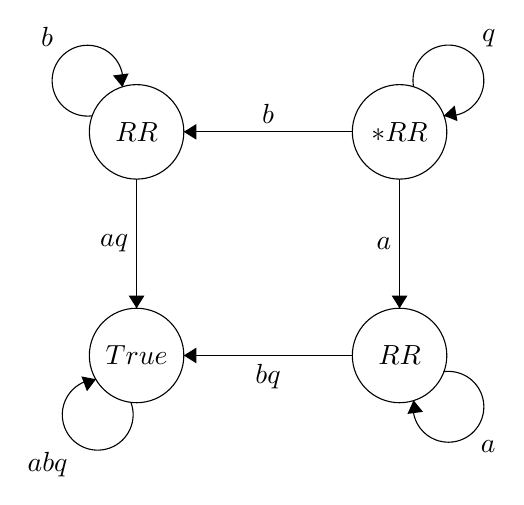
\begin{tikzpicture}[scale=0.2]
    \tikzstyle{every node}+=[inner sep=0pt]
    \draw [black] (54,-42.2) circle (3);
    \draw (54,-42.2) node {$RR$};
    \draw [black] (37.3,-28) circle (3);
    \draw (37.3,-28) node {$RR$};
    \draw [black] (37.3,-42.2) circle (3);
    \draw (37.3,-42.2) node {$True$};
    \draw [black] (54,-28) circle (3);
    \draw (54,-28) node {$*RR$};
    \draw [black] (56.805,-43.229) arc (97.58097:-190.41903:2.25);
    \draw (59.62,-47.57) node [below] {$a$};
    \fill [black] (54.89,-45.05) -- (54.5,-45.91) -- (55.49,-45.78);
    \draw [black] (34.491,-26.979) arc (277.76012:-10.23988:2.25);
    \draw (31.61,-22.64) node [above] {$b$};
    \fill [black] (36.4,-25.15) -- (36.79,-24.29) -- (35.8,-24.42);
    \draw [black] (51,-42.2) -- (40.3,-42.2);
    \fill [black] (40.3,-42.2) -- (41.1,-42.7) -- (41.1,-41.7);
    \draw (45.65,-42.7) node [below] {$bq$};
    \draw [black] (37.3,-31) -- (37.3,-39.2);
    \fill [black] (37.3,-39.2) -- (37.8,-38.4) -- (36.8,-38.4);
    \draw (36.8,-35.1) node [left] {$aq$};
    \draw [black] (51,-28) -- (40.3,-28);
    \fill [black] (40.3,-28) -- (41.1,-28.5) -- (41.1,-27.5);
    \draw (45.65,-27.5) node [above] {$b$};
    \draw [black] (54,-31) -- (54,-39.2);
    \fill [black] (54,-39.2) -- (54.5,-38.4) -- (53.5,-38.4);
    \draw (53.5,-35.1) node [left] {$a$};
    \draw [black] (54.889,-25.147) arc (190.43418:-97.56582:2.25);
    \draw (59.67,-22.63) node [above] {$q$};
    \fill [black] (56.81,-26.97) -- (57.68,-27.32) -- (57.5,-26.33);
    \draw [black] (36.935,-45.166) arc (20.7166:-267.2834:2.25);
    \draw (31.65,-48.34) node [below] {$abq$};
    \fill [black] (34.72,-43.71) -- (33.8,-43.53) -- (34.15,-44.47);
    \end{tikzpicture}
    \end{center}

    This is an epistemic model: NO \\
    This is a doxasic model: YES \\

    \item The update product of the two models \textbf{M} $\bigotimes$ $\Sigma$ : \\

    This is an epistemic model: YES / NO \\
    This is a doxasic model: YES / NO \\

\end{enumerate}


%%%%%%%%%%%%%%%%
%% Exercise 2 %%
%%%%%%%%%%%%%%%%
\section{Exercise 2}

\begin{enumerate}

    \item There are ? possible worlds.
    \item
    \item
    \item
    \item

\end{enumerate}


%%%%%%%%%%%%%%%%
%% Exercise 3 %%
%%%%%%%%%%%%%%%%
\section{Exercise 2}

\begin{enumerate}

    \item
    \item
    \item
    \item
    \item
    \item
    \item
    \item
    \item

\end{enumerate}


\end{document}


